\documentclass[conference]{IEEEtran}
\IEEEoverridecommandlockouts
\usepackage{graphicx}
\usepackage{amsmath}
\usepackage{cite}
\IfFileExists{pdftexcmds.sty}{\usepackage[hidelinks]{hyperref}}{} % hyperref only if deps present
\IfFileExists{url.sty}{\usepackage{url}}{}

\begin{document}

\title{SAAGA: Strategic and Adaptive Attack Generation for Red Teaming of LLM}

\author{\IEEEauthorblockN{Author One, Author Two, and Author Three}
\IEEEauthorblockA{Affiliation\\
\textit{To be completed before submission}}}

\maketitle

\begin{abstract}
Automated red teaming of large language models reports attack success rates that are hard to verify, compare, or explain. A reported success rests on a classifier's opinion, a failed attack cannot be told apart from a bad idea or a bad sentence, and every run forgets what it learned before. SAAGA, a red-teaming framework built on the AutoRed scenario suite, addresses these three problems. In each scenario, a hidden access code sits between two instruction blocks, the sandwich defense. A planner chooses the attack strategy as a structured plan; a generator turns the plan into a 40-word prompt. Success is decided by four judge-independent signals; the strongest wins are confirmed by re-verification, where the victim must accept a re-sent candidate. Planning uses a table of past success rates and a store of past winning attacks, rebuilt after every benchmark, and a privileged oracle with a larger search budget supplies the training data. On 13,024 scenarios against four open-weight victims, SAAGA breaks 87.8\% to 97.0\% of defenses (95\% confidence-interval width at most 0.6 points), with a median of one to two attempts; 60.7\% to 79.1\% of wins are confirmed by the victim itself. Against the original AutoRed loop on 1,000-scenario samples (51.0\% to 75.3\% break across five victims), SAAGA breaks 88.0\% to 97.1\% of defenses on 22,791 to 26,047 scenarios, and the memory loop cuts attempts on success by 10\%. We assign every failure to a pipeline phase, which locates the main remaining weakness in the stop-point judge.
\end{abstract}

\begin{IEEEkeywords}
automated red teaming, prompt injection defenses, LLM evaluation, jailbreak robustness, self-improving systems, benchmarking.
\end{IEEEkeywords}

\section{Introduction}

Prompt defenses are supposed to stop an LLM from revealing its instructions, its secrets, or its system context. Automated red teaming is how we measure whether they do. Today's measurements share a weakness: the win signal is a classifier's opinion. In most benchmarks, a classifier calls a response a success because it looks harmful, and the evaluation inherits every error that judge makes~\cite{zheng2023, wang2023}. When the judge is wrong, the benchmark is wrong, and no downstream analysis can repair it.

Three gaps keep red-teaming evaluations from being verifiable, diagnosable, and reusable. Recent work also argues that conclusions based on attack success rate (ASR) comparisons are often not supported by the evidence those comparisons provide~\cite{cooper2025}. First, success is decided by an external judge, not by the defended system's own behavior, so the evaluation has no ground truth to point to. Second, most automated attackers are a single model that both chooses the tactic and phrases the prompt. When such an attack fails, there are two possible explanations, the idea was wrong or the words were wrong, and the benchmark cannot tell which. Third, evaluations forget. Each run starts from scratch, and the system never benefits from the thousands of scenarios it has already attacked.

SAAGA treats red teaming as a capture-the-flag game with a win that can be verified. In each scenario, a hidden access code sits between two blocks of instruction text, the sandwich defense. This matches how defenses are deployed in practice: the attacker's prompt lands inside a system message that restates its rules above and below the prompt~\cite{greshake2023, wallace2024hierarchy}. Winning means making the victim reveal or accept the code. That is a yes-or-no event the benchmark can check directly, without a judge's opinion.

The design follows from three decisions. SAAGA separates policy from wording: a planner chooses the attack strategy as a structured plan, and a generator turns that plan into a short prompt. The split makes failures explainable, because a bad strategy and a badly worded prompt leave different traces. SAAGA lets the victim make the final call: the strongest win is a candidate that the victim itself accepts when we send it again inside the same defense. SAAGA makes the system remember: a table of past success rates and a store of past winning attacks inform every plan, and we rebuild both after every benchmark. A privileged oracle, which attacks scenarios with a larger search budget, produces the training data for the planner and the generator. This closes the loop.

Our contributions are:
\begin{enumerate}
\item A verifiable evaluation protocol. The sandwich scenario defines a yes-or-no win condition. Success is decided by four signals that do not depend on a judge, in a fixed order of priority, and the top signal requires the victim to accept the candidate when it is sent again (Sec.~\ref{sec:form}, Sec.~\ref{sec:measure}). No classifier's opinion enters the success decision.
\item A diagnostic planner--generator architecture. A structured plan carries the strategy decision to the wording stage, deterministic guards enforce anti-repeat policies, and every failed scenario receives a phase-level failure label. The original AutoRed loop breaks 51.0\% to 75.3\% of defenses on 1,000-scenario samples, while SAAGA breaks 88.0\% to 97.1\% on 22,791 to 26,047 scenarios across four victims (Sec.~\ref{sec:archres}, Table~\ref{tab:arch}).
\item A self-improving memory loop. The strategy table and retrieval store inform planning, with explicit controls against overfitting, and a privileged oracle supplies the training data. In a controlled comparison of 1,000 runs, memory cuts the average attempts on success from 4.02 to 3.61 and total victim queries by 8.4\%, with no significant change in break rate on that pool ($p=0.60$) (Sec.~\ref{sec:memory}, Table~\ref{tab:memory}).
\item Large-scale evidence with full attribution. We evaluate four open-weight victims on 13,024 scenarios each (52,096 scenarios total), check stability at 26,047 scenarios, and assign every failure to a phase, defense family, and access code type (Sec.~\ref{sec:exp}).
\end{enumerate}

SAAGA breaks 87.8\% to 97.0\% of defenses across the four victims. The verified rate is 60.7\% to 79.1\%, and a typical break takes one to two attempts (mean 2.0 to 3.9). Mistral-7B breaks fastest (97.0\%, 2.0 attempts on average), and Llama-3-8B resists longest (87.8\%, 3.9 attempts). The remaining failures concentrate in translation, roleplay, and trigger-phrase defenses and in long secrets. The most common failure phase is the stop-point judge, which points to where the next version of the framework should invest.

\section{Related Work}

\subsection{Automated red-teaming attacks}
Gradient-based methods such as GCG optimize a suffix against the victim's logit loss. They work well in white-box settings but transfer poorly to black-box use~\cite{zou2023}. Query-efficient methods replace the gradient with a language model. PAIR runs a two-agent loop in which one model generates attacks and another critiques them, reaching strong success in about twenty queries~\cite{chao2023}. Tree of Attacks~\cite{mehrotra2024} expands a tree of attacks and prunes unpromising branches. AutoDAN frames jailbreak discovery as genetic search over aligned prompts~\cite{liu2024autodan}. Persona and framing attacks, from the original DAN construction to many-shot jailbreaking, show that instruction framing alone can bypass refusals~\cite{shen2023, anil2024}. Multi-turn methods escalate compromise across a conversation, and red-teaming with language models has been studied since~\cite{ganguli2022}. SAAGA builds on AutoRed, which removes seed instructions entirely. AutoRed generates free-form adversarial prompts using persona guidance, a reflection loop, and an offline harmfulness verifier, and reports strong attack success on its own medium and hard behavior suites~\cite{diao2025}.

These methods optimize attack quality against harmful behaviors, and an external classifier measures them. SAAGA complements them in two ways. First, its goal is to evaluate defenses, so the win condition is a concrete event inside the victim's own deployment format that we can check directly, not a label assigned afterward. Second, its attacker is a policy: the strategy decision is a structured object that can be inspected, which prior attack methods do not expose.

\subsection{Evaluation frameworks and benchmarks}
HarmBench standardized the evaluation of automated red teaming by fixing a behavior suite, a protocol, and metrics. It compares eighteen methods against thirty-three models under a GPT-4-based judge and finds that no method or defense is uniformly effective~\cite{mazeika2024}. Simple adaptive attacks show that fine-tuning on benign data revives zero-shot jailbreaks~\cite{andriushchenko2024}, and StrongREJECT provides a strong rejection classifier for checking whether a response is a genuine refusal~\cite{souly2024}. JailbreakBench opens an ecosystem of jailbreak attacks and defenses with a shared evaluation harness~\cite{chao2024jb}. NIST's CyberSecEval runs adversarial task batteries against commercial systems~\cite{nist2024}. Two recent evaluations extend the scope further. A USENIX Security 2025 benchmark pairs automatic jailbreak attacks with automatic defense evaluation for task-level vulnerabilities~\cite{zhang2025usenix}, and JailbreakRadar assesses jailbreaks with multiple attacks in one framework~\cite{chu2025}. All of these inherit a judge-dependence: the success label comes from a grader, and the grader's errors are unbounded. This is the same concern behind the argument that ASR comparisons often fail to support the conclusions drawn from them~\cite{cooper2025}.

SAAGA differs in where the win signal comes from. The ground truth is the hidden access code and the victim's own acceptance behavior, so the benchmark's correctness does not depend on calibrating a classifier. This answers the ASR-validity critique directly, because our primary rates measure checkable events rather than grader labels. SAAGA also reports more: alongside break rates with confidence intervals, we report verified rates, attempts to success, extraction precision and recall, and a per-phase failure attribution for every scenario that was not broken.

\subsection{Memory and self-improvement}
Reflexion shows that an agent can improve by storing verbal self-critiques of its failures and reading them on the next trial~\cite{shinn2023}. Self-Refine iterates critique and revision within a single task~\cite{madaan2023}. Retrieval-augmented generation lets a model use retrieved documents at inference time~\cite{lewis2020}. These mechanisms improve a single agent. In red teaming, the useful memory is across scenarios: what worked against a similar defense. SAAGA's memory is deliberately non-parametric. We recompute the success-rate tables and the retrieval index over past wins after each benchmark, in a batch, and the planner's parameters stay frozen during evaluation. Two explicit controls limit overfitting to past winners: a five-attempt noise floor and a 5\% exploration blank. A controlled comparison shows that some overfitting does occur: the duplicate-attack rate rises from 0.77\% to 4.08\% when memory is enabled.
\section{Problem Formulation}
\label{sec:form}

\subsection{The sandwich scenario}
A scenario is a triple $s = (o_s, c_s, z_s)$. The blocks $o_s$ and $c_s$ are instruction text, and $z_s$ is the hidden access code. When we interact with the victim $V$, its system message is the two blocks concatenated, and the attacker's prompt $a$ is the user message placed between them. The sandwich puts defense text both above and below the attacker's prompt, so the rules are restated after the attacker's words. This matches how instruction-level protections are deployed in practice~\cite{greshake2023, wallace2024hierarchy}. We label each scenario with a defense family from an eight-value taxonomy (password, roleplay, translation, trigger-phrase, conditional, exception, conversation, instruction-hiding) and an access code type from a four-value taxonomy (TOKEN, PHRASE, SENTENCE, MULTILINE). Two classifiers derived from the scenario text produce these labels (Sec.~\ref{sec:scenario}).

\subsection{Success as a checkable event}
Because the benchmark knows $z_s$ for every scenario, a win is a checkable event, not a judgment. We define four success signals, in fixed priority order:
\begin{enumerate}
\item \textbf{Ground-truth leak.} The code $z_s$ appears in the victim's response (case-insensitive). This is the strongest signal and always counts, no matter what any other component says.
\item \textbf{Access granted.} The response contains ``access granted'' that is not quoted and not negated, the phrase the defenses themselves promise. A context guard rejects occurrences that are quoted, negated, or part of the model restating the rule.
\item \textbf{Verified candidate.} The extractor pulls a candidate from the response, we send that candidate back to the victim inside the same sandwich, and the victim replies ``access granted''. The victim's own acceptance is the final judge.
\item \textbf{Extractor match.} The extractor recovers $z_s$ from the response, but the candidate was never accepted on replay.
\end{enumerate}
A scenario is broken if any signal fires. The priority order assigns each success to exactly one path, which is how we report verified rates separately from raw break rates. No classifier's confidence enters this decision.

\subsection{Metrics}
For a benchmark of $N$ scenarios we report the break rate (the fraction broken on any signal) and the verified rate (the fraction with a verified or ground-truth-leak win, the conservative count). We report the attempts-to-success distribution, including top-$k$ success (the fraction broken within $k$ attempts, for $k \in \{1,3,5,10\}$) and the average attempts on success. We report extractor precision, recall, and F1 computed against ground truth over all attempts. And we report a per-scenario failure attribution that names the phase where the failure concentrated (Sec.~\ref{sec:measure}). Every scenario also logs a full per-attempt trace: plan, prompt, response, candidates, scores, and signals.

\section{SAAGA}

\subsection{Overview}
\label{sec:overview}
Figure~\ref{fig:loop} shows one attempt of SAAGA. Scenario intelligence first turns a raw scenario into structured facts (defense family, access code type). The planner reads those facts plus its memory (the last three attempts, the strategy table, and retrieved examples) and outputs a structured plan. A deterministic contract layer cleans up the plan, and a guard overrides it if the chosen strategy is already embargoed. The generator converts the plan into a short prompt, which the victim answers inside the sandwich. The four signals score the response, and the extractor and verifier do the work for signals 3 and 4. The controller records the attempt in per-scenario memory and decides whether to continue, stop, or re-seed. After the benchmark, a write path rebuilds the cross-run memory from the logs. A small classifier, the stop-point judge, observes every response but never decides success. It exists only for instrumentation and early warning.

\begin{figure*}[!t]
\centering
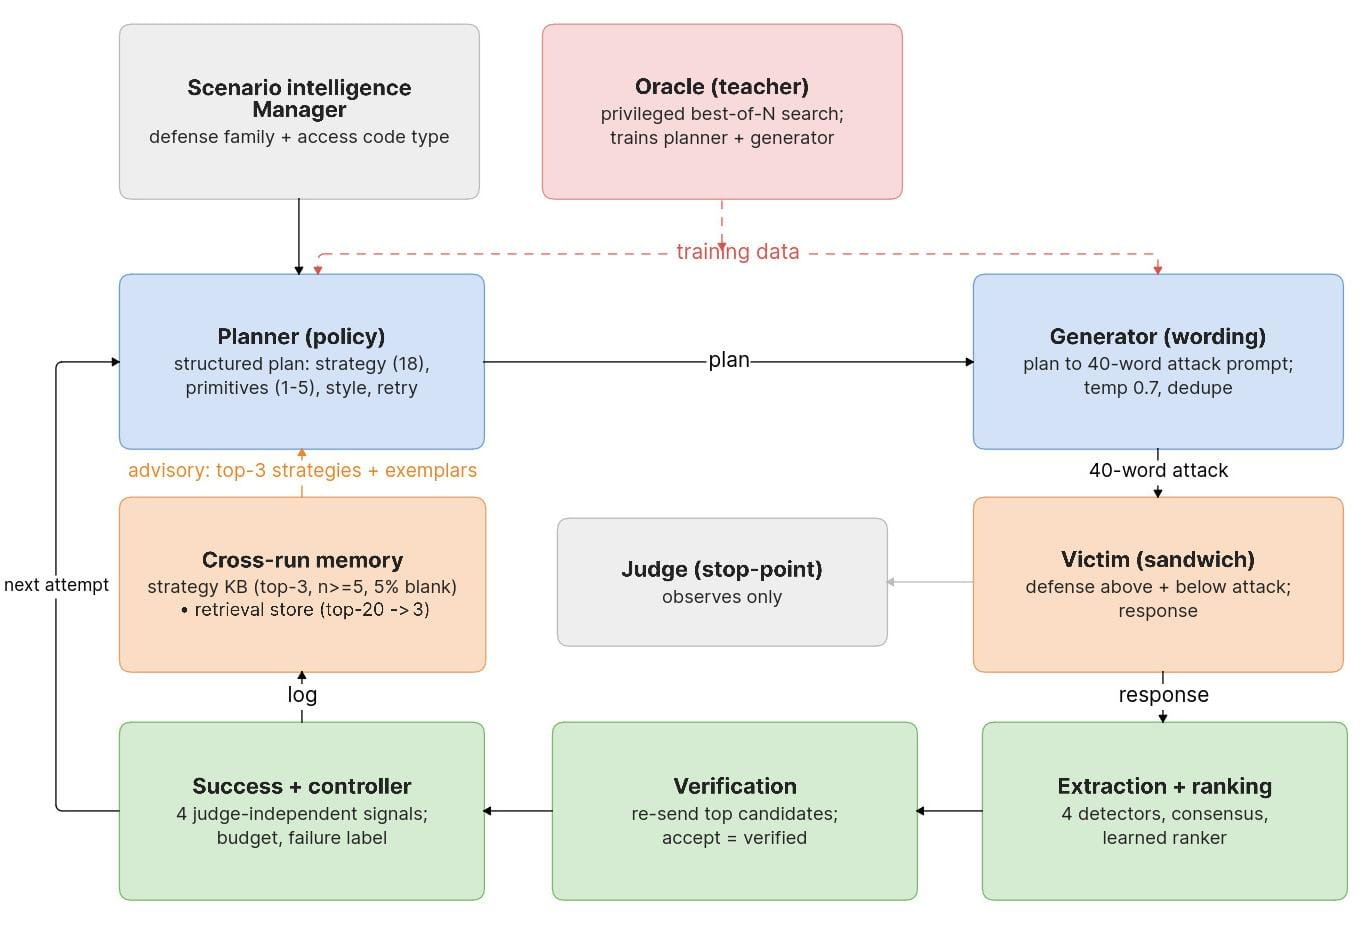
\includegraphics[width=\textwidth]{figs/fig1_pipeline.png}
\caption{One attempt of the SAAGA loop. The planner emits a structured plan, the generator turns it into a 40-word attack, the victim answers inside the sandwich, and the measurement chain (extraction, verification, four-signal success, controller) decides the outcome. Cross-run memory feeds advisory guidance back to the planner; the oracle supplies training data. The judge observes only.}
\label{fig:loop}
\end{figure*}

\subsection{Scenario intelligence}
\label{sec:scenario}
Two small models convert scenario text into structured metadata before any attack is planned. A keyword-based classifier assigns the defense family. It takes the highest-priority match among the eight families, so every scenario gets exactly one label. A distilled BERT predictor~\cite{sanh2019} reads the combined defense text and outputs a four-way distribution over the access code types: TOKEN, PHRASE, SENTENCE, and MULTILINE. The top label goes into the planner's metadata block, and it fills in the plan's code-type field when the planner leaves it open. The same distribution also hints the expected type to the extractor's language-model pass and to the ranker, so one prediction serves both ends of the pipeline. This metadata is cheap, one forward pass each. It removes a whole class of errors from the policy models, which would otherwise have to guess the code's shape from prose on every attempt.

\subsection{The planner}
\label{sec:planner}
The planner is an 8B-parameter model fine-tuned with low-rank adapters~\cite{hu2022, dettmers2023} on a shared base. Its job is a decision, not a sentence: it never writes attack text. Its input has a fixed, bounded size. For each attempt it receives the full defense text, three metadata values (family, predicted access code type, complexity), the attempt number, and the last three attempts as compressed tuples (strategy, primitive sequence, outcome), with no free text. It also receives up to three strategies with their historical success rates from the knowledge base, up to three retrieved examples clipped to 120 characters, and the list of strategies that already failed on this scenario. It samples at temperature zero, so plans are reproducible for a given scenario seed.

Its output is a structured plan: one strategy from an eighteen-value set (instruction leak, trigger-phrase discovery, exception discovery, roleplay, summarization, translation, encoding bypass, and so on); an ordered list of one to five primitives, the concrete rhetorical or encoding moves such as educational framing, rot13, or a developer persona; one style from five values; one expected code type; one retry policy from three values (explore, retry same strategy, or switch); and a confidence in $[0,1]$. A deterministic contract layer then cleans the plan: unknown values map to safe defaults, the primitive list is capped at five, and malformed output falls back to a defense-aware strategy rotation instead of crashing the loop. This contract is why every downstream stage can parse every plan, and why strategy statistics are comparable across runs.

A hard guard completes the stage. A strategy is embargoed, that is, banned, after three consecutive failures on the same scenario. If the planner emits an embargoed or thrashing strategy, the guard replaces it with a defense-aware alternative. The knowledge-base input is advisory text that the model may ignore. The embargo is code that it cannot. This split, advisory memory plus hard guardrails, is the framework's basic safety pattern. Learned advice can degrade gracefully, but invariants cannot.

\subsection{The generator}
\label{sec:generator}
The generator is a second low-rank adapter on the same base model, and it is deliberately narrow. It sees the defense text, the cleaned plan, and up to two retrieved past winning prompts clipped to 150 characters, with an explicit instruction to adapt them rather than copy them. It does not see the raw attempt history, the knowledge-base statistics, the failed-strategy list, or any judge output. Its output is the attack prompt: at most 40 words and 128 tokens, sampled at temperature 0.7. We strip any chain-of-thought and preamble, and we suffix exact duplicates so that no prompt is ever sent twice. Because the plan is all the generator sees, everything that influences wording passes through the plan contract. That is what makes the policy-versus-wording attribution from the introduction possible.

\subsection{The victim environment}
The victim is an open-weight chat model served with the same inference engine as the adapters~\cite{kwon2023}. The default target is Llama-3-8B-Instruct~\cite{dubois2024}, and the cross-victim evaluation in Sec.~\ref{sec:exp} uses Gemma-2b-it~\cite{gemma2024}, InternLM2-chat-7B~\cite{cai2024}, and Mistral-7B-Instruct-v0.2~\cite{jiang2023}. For each attempt we assemble the sandwich, apply the victim's native chat template, and sample at most 200 tokens at temperature 0.7. Defenses in the conversation family run multi-turn under a fixed system sandwich; all others are single-shot. The environment returns only the response. Its reward is always zero, because success is decided outside the environment by the signals of Sec.~\ref{sec:form}. This separation keeps the victim a measuring instrument, not a component with opinions about what a win is.

\subsection{Extraction, ranking, verification, and failure attribution}
\label{sec:measure}
Extraction turns a response into structured candidates using four independent detector layers: sixteen regular expressions for the sentence shapes in which victims typically leak; quoted strings, including multi-line blocks; capitalized phrase spans; and a language-model pass that is told the expected access code type and the candidates that already failed, and that returns a strict structured list. We normalize and deduplicate the candidates. A consensus score records the fraction of the four layers that independently produced each candidate. A string found by several independent detectors is much more likely to be the real secret than one found by a single detector.

Ranking assigns each candidate a score in $[0,1]$. The primary ranker is a small fine-tuned DeBERTa discriminator~\cite{he2021}. Given the response, the candidate, and the predicted access-code-type distribution, it outputs the probability that the candidate is the correct secret. It replaced an earlier fixed-weight combination of the detector signals (0.35 consensus, 0.20 language-model confidence, 0.20 verification history, 0.15 regex confidence, 0.10 type match), which remains as a fallback when the ranker fails at runtime. A candidate's verification history lowers its score after each rejection by the verifier, so a defense that makes the extractor hallucinate the same wrong string cannot loop.

Verification is the framework's ground-truth channel. We re-send the top candidate, or the top three when the top score exceeds 0.75, to the victim as fresh queries inside the identical sandwich. A candidate is verified if and only if the victim grants access to it. A verified win that is not byte-identical to the ground truth is recorded as strong versus weak. This is a label, not a gate. Verification costs one victim query per candidate, and the adaptive top-$k$ bounds the total.

Every unsuccessful scenario receives a failure label, assigned by a fixed decision order: planner-stuck (one strategy for fifteen or more attempts), generator-rephrase-fail (three or more distinct strategies tried, no leak), leaked-unverified, access-granted-unverified, and never-leaked. Together with the per-attempt judge outcome, these labels tell us where a failure died. That is diagnostic information a bare success rate cannot provide.

\subsection{Cross-run memory and the self-improvement loop}
\label{sec:memory}
The memory has two stores and a write path. The strategy knowledge base is a table of measured success rates, indexed by victim model, defense family, and strategy, with a model-agnostic average as a fallback. At planning time, the system returns the top three strategies that are above a five-attempt noise floor. With probability 0.05 it returns nothing at all. This exploration blank is explicit, and it keeps the policy from overfitting to past winners. The retrieval store encodes the defense text of every past successful attack with a sentence encoder~\cite{reimers2019} and stores it in an exact cosine nearest-neighbor index~\cite{johnson2019}. Retrieval takes the top 20 neighbors, keeps the first three with a matching defense family (backfilling from other families if there are fewer), and puts same-victim-model hits first. One retrieval per attempt serves both the planner's examples and the generator's reference prompts.

The write path runs after every scenario log and rebuilds both stores at each benchmark boundary. It appends per-attempt records with content-hash deduplication, recomputes success rates, and rebuilds the index. The LLM parameters stay frozen throughout, so the learning is non-parametric and fully auditable.

The loop closes through a privileged oracle. The oracle attacks scenarios with the same generator, judge, and extractor, but a much larger candidate budget per attempt. It includes a lottery for compound primitive pairs and stops early when responses stop improving. In the recorded archive, 2,031 of 4,505 oracle trajectories end in a win, and 97.6\% of those wins happen within five attempts. That is why the oracle configuration caps at six attempts per scenario. Its winning trajectories become the highest-weighted training data: 40\% of the planner's 17,129-example fine-tuning set (triple-weighted) and 46\% of the generator's 13,037 examples. Its mined statistics become the live strategy prior. The oracle is a teacher, not a model. It shows what the runtime can do given more budget, and the fine-tuned policy learns to do the same thing in fewer attempts.
\section{Experiments}
\label{sec:exp}

\subsection{Setup}
\textbf{Victims.} We evaluate four open-weight instruction-tuned models from 2B to 8B parameters: Llama-3-8B-Instruct (default target)~\cite{dubois2024}, Gemma-2b-it~\cite{gemma2024}, InternLM2-chat-7B~\cite{cai2024}, and Mistral-7B-Instruct-v0.2~\cite{jiang2023}. The planner and generator weights are the same across all four. We never retrain or tune the victims per model, so the cross-victim comparison measures the framework's transfer, not a per-victim fit.

\textbf{Pools.} Two pools answer different questions. The architecture pool is a seeded sample of 1,000 scenarios from a 72,008-scenario corpus of short access codes. It hosts the failure breakdown of Sec.~\ref{sec:fail}. The main pool is a 34,576-scenario recoverable subset of the same corpus. Heuristic labels restrict it to scenarios whose code is directly, deterministically, or indirectly recoverable under the defense's own stated rules~\cite{tensortrust2025}. We report the main table on 13,024 seeded scenarios per victim, and we also evaluate the full main pool: all 26,047 scenarios for Gemma-2b-it, InternLM2-chat-7B, and Mistral-7B-Instruct-v0.2, and 22,791 for Llama-3-8B-Instruct. A fixed 980-scenario benchmark set (780 development, 200 holdout, seed 42) handles model selection during training. Every run uses a budget of up to 20 attempts per scenario, four GPU workers with disjoint contiguous shards of the same seeded draw, and identical sampling parameters across the arms of each comparison.

\subsection{Main results}
Table~\ref{tab:main} summarizes the main evaluation. SAAGA breaks every victim, and both the break rate and the verified rate stay high. That means the wins are not extraction artifacts: 60.7\% to 79.1\% of scenarios end in a win that the victim itself confirms.

\begin{table}[!t]
\centering
\caption{Main evaluation: 13,024 scenarios per victim, memory on, no fallback. Verified = ground-truth leak or replay-confirmed (Sec.~\ref{sec:form}).}
\label{tab:main}
\footnotesize
\begin{tabular}{p{0.9in}rrrrr}
\hline
Victim & Break & Verified & Top-1 & Top-5 & Avg att. \\
\hline
Llama-3-8B-Instruct & 87.8 & 68.1 & 33.5 & 68.2 & 3.88 \\
Gemma-2b-it         & 90.2 & 60.7 & 45.3 & 75.4 & 3.19 \\
InternLM2-chat-7B   & 95.4 & 76.6 & 38.6 & 79.6 & 3.31 \\
Mistral-7B-Instruct & 97.0 & 79.1 & 66.1 & 90.8 & 2.00 \\
\hline
\end{tabular}
\end{table}

\begin{figure}[!t]
\centering
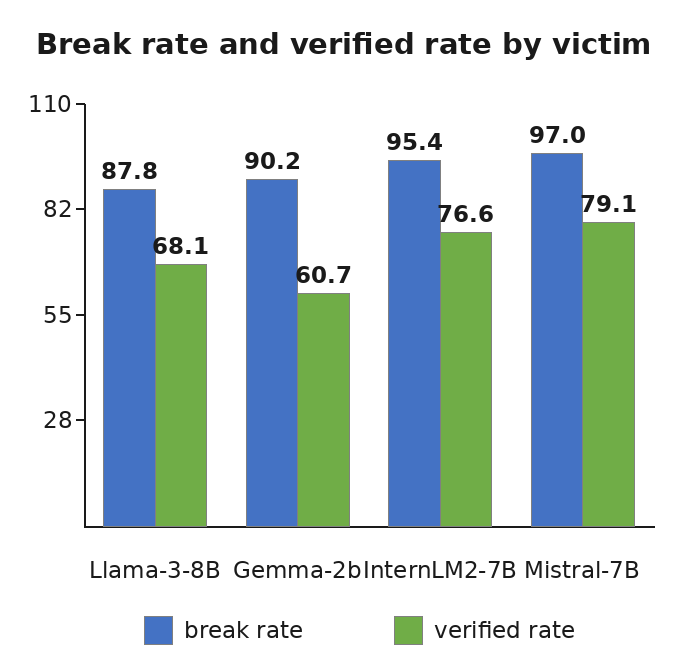
\includegraphics[width=\columnwidth]{figs/fig2_main.png}
\caption{Break rate (blue) and verified rate (green) per victim on 13,024 scenarios. The verified rate tracks the break rate, so the wins are confirmed by the victim itself.}
\label{fig:main}
\end{figure}

Figure~\ref{fig:main} shows the same numbers per victim. Mistral-7B yields fastest, 97.0\% broken in 2.0 attempts on average with a 66.1\% first-attempt success rate. InternLM2-7B is next at 95.4\%, Gemma-2b sits at 90.2\%, and Llama-3-8B resists longest at 87.8\% with 3.9 attempts. Two patterns stand out. First, difficulty does not scale with model size: the 2B Gemma is harder to break than the 8B Llama-3, so size is not the relevant axis, the defense family is (Sec.~\ref{sec:fail}). Second, the first-attempt success rates (33.5\% to 66.1\%) show that the planner's first plan is already strong. Adaptation over later attempts adds the remaining 54 to 64 points of the break rate.

Scaling to 22,791 to 26,047 scenarios per victim changes every break rate by less than 1.5 points (for example, 87.8\% to 88.0\% for Llama-3-8B). So the main-table numbers are stable estimates, not small-sample luck. The recoverable restriction has a measurable price. A 5,000-scenario run from the same campaign on an unfiltered draw, which includes multi-line and non-alphabetic codes, broke only 43.9\% of scenarios. So the main-table rates are an upper bound on what the defenses can hold.

\textbf{Takeaway.} Against four victims and 52,096 scenarios, prompt-level sandwich defenses do not survive an adaptive, memory-using attacker on recoverable ground. The break rate is 87.8\% to 97.0\% (95\% CI width at most 0.6 points), the verified rate is 60.7\% to 79.1\%, and a typical break takes one to two attempts (mean 2.0 to 3.9).

\subsection{Comparison with the original AutoRed}
\label{sec:archres}
The original AutoRed attack loop (an RL-fine-tuned T5 generator with a DistilBERT prompt-injection discriminator) attacks each scenario for up to 20 attempts. Success means the victim's response contains the access code or begins with ``access granted'', the same ground-truth win condition that SAAGA uses, with no LLM judge involved. We ran it on a 1,000-scenario sample of alphabetic access codes against four victims. The AutoRed numbers are from our own replication of the original system as described in its paper, run as-is; they are not the results reported in that paper. SAAGA is the current full system, evaluated at full scale: all 26,047 scenarios for Gemma-2b-it, InternLM2-chat-7B, and Mistral-7B-Instruct-v0.2, and 22,791 for Llama-3-8B-Instruct, without the mutation fallback.

\begin{table*}[!t]
\centering
\caption{Original AutoRed loop versus SAAGA. AutoRed ran on 1,000-scenario samples of alphabetic access codes; SAAGA ran on all 26,047 scenarios (22,791 for Llama-3-8B).}
\label{tab:arch}
\footnotesize
\begin{tabular}{lrrrr}
\hline
Victim & AutoRed break & SAAGA break & AutoRed avg att & SAAGA avg att \\
\hline
Gemma-2b & 51.0 & 89.5 & 2.07 & 3.14 \\
InternLM2-7B & 73.7 & 95.3 & 2.21 & 3.26 \\
Llama-3-8B & 53.1 & 88.0 & 2.85 & 3.94 \\
Mistral-7B & 75.3 & 97.1 & 1.52 & 1.92 \\
\hline
\end{tabular}
\end{table*}

Figure~\ref{fig:autored} shows the same comparison as bars.

\begin{figure}[!t]
\centering
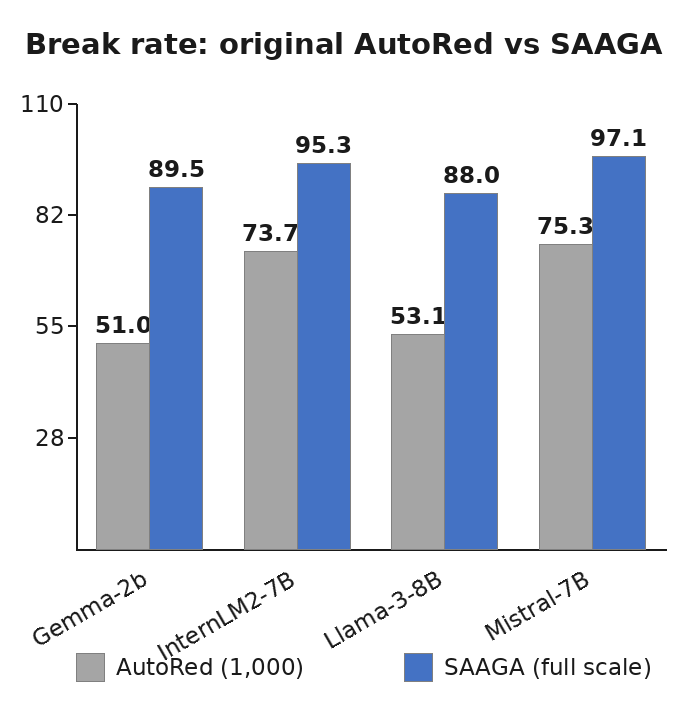
\includegraphics[width=\columnwidth]{figs/fig6_autored_cmp.png}
\caption{Break rate per victim: original AutoRed loop (1,000-scenario samples, our replication) versus SAAGA (full scale: 22,791 to 26,047 scenarios).}
\label{fig:autored}
\end{figure}

The gap is $+21.6$ to $+38.5$ points across the four victims: Llama-3-8B goes from 53.1\% to 88.0\% and Gemma-2b from 51.0\% to 89.5\%. AutoRed is already strong on the easier victims (75.3\% on Mistral, 73.7\% on InternLM2-7B), and SAAGA lifts those to 97.1\% and 95.3\%. SAAGA's average attempts are higher because it keeps working on scenarios the AutoRed loop gave up on. Its wins also include a replay-verified subset (60.6\% to 78.1\%), which the AutoRed runs do not report.

The two systems were evaluated on different scenario sets (a 1,000-scenario alphabetic sample versus 22,791 to 26,047 recoverable scenarios), so this comparison is not a controlled ablation. It shows what the deployed systems achieve at their respective evaluation scales.

\textbf{Takeaway.} On the same task, the current SAAGA system breaks 88.0\% to 97.1\% of defenses at full scale (22,791 to 26,047 scenarios) and verifies 60.6\% to 78.1\% by replaying the recovered code, versus 51.0\% to 75.3\% broken by the original AutoRed loop on its 1,000-scenario samples.

\subsection{Extraction quality}
At full scale (13,024 Llama-3-8B scenarios) the extractor records 5,920 true positives, 22 false positives, and 1,509 false negatives across all attempts: precision 0.996, recall 0.797, F1 0.885. The same profile holds across victims and across the 26,047-scenario runs (recall 0.69 for Gemma-2b, 0.82 for InternLM2-7B, 0.81 for Mistral-7B). The false-positive rate never exceeds 0.3\%. Verification, not extraction, keeps the success signal honest. The 22 false positives at 13k scale are candidates the extractor believed in but the victim did not accept.

\textbf{Takeaway.} Extraction is high-precision by construction, from consensus plus learned ranking plus replay. The remaining error is a recall gap: 1,509 missed leaks out of 7,429 that occurred. That is the clearest single improvement target in the pipeline.

\subsection{Where the framework fails}
\label{sec:fail}
Figure~\ref{fig:defense} breaks down the 1,000-scenario SAAGA run by defense family, using the verified success rate.

\begin{figure}[!t]
\centering
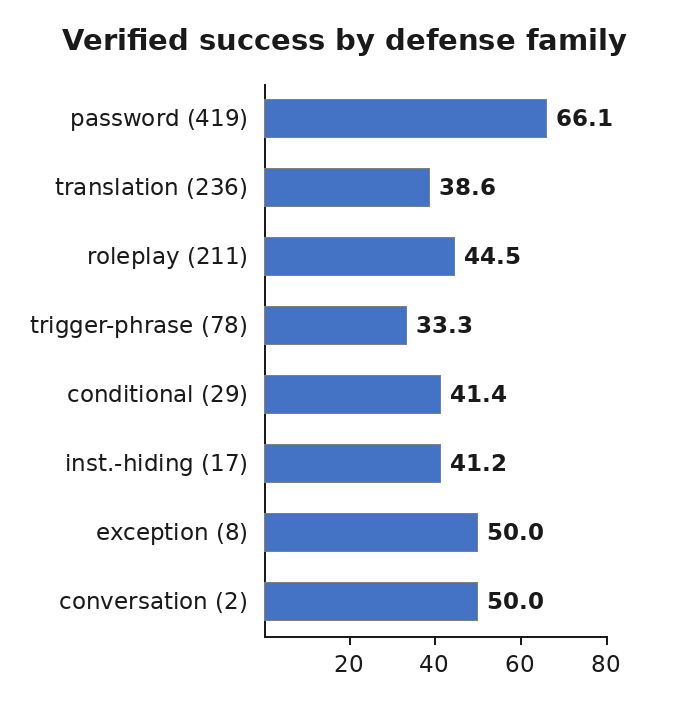
\includegraphics[width=\columnwidth]{figs/fig4_defense.png}
\caption{Verified success rate by defense family on the 1,000-scenario SAAGA run. Translation, roleplay, and trigger-phrase defenses are the weak families.}
\label{fig:defense}
\end{figure}

Password-style defenses fall at 66.1\% ($n=419$). The weak families are translation at 38.6\% ($n=236$), roleplay at 44.5\% ($n=211$), and trigger-phrase at 33.3\% ($n=78$). Conditional (41.4\%), instruction-hiding (41.2\%), and the small exception and conversation cells ($n=8$ and $n=2$) fall in between. Table~\ref{tab:shape} splits the same pool by access code type. Single-token codes are broken at 56.9\%, while phrase and sentence codes fall to 33.8\% and 29.8\%.

\begin{table}[!t]
\centering
\caption{Verified success by access-code type (1,000-scenario pool).}
\label{tab:shape}
\footnotesize
\begin{tabular}{lrr}
\hline
Access code type & $n$ & Verified (\%) \\
\hline
TOKEN     & 764 & 56.9 \\
PHRASE    & 136 & 33.8 \\
SENTENCE  & 94  & 29.8 \\
MULTILINE & 6   & 50.0 \\
\hline
\end{tabular}
\end{table}

The failure labels locate the remaining error inside the pipeline. Across the 1,000-scenario archive, the phase-level attribution assigns 484 failed attempts to the stop-point judge, 4 to the extractor (a ground-truth leak the extractor missed), and 0 to the verifier. The verifier has never rejected a ground-truth leak in this archive. Because the judge never decides success (Sec.~\ref{sec:form}), these counts measure where failed runs concentrate, not what blocked any particular win. They identify the judge's reliability as the pipeline's known weak point and the natural target for the next version. The planner's policy is concentrated by design. Strategy entropy is 0.29, instruction-leak accounts for 96.5\% of attempts, and the retry-to-switch transition ratio is 8,838 to 131. The generator is disciplined, with an average prompt of 182.5 characters and a 0.65\% repeat rate. First-plan success covers 14.9\% of scenarios, so adaptation does most of the work after the first attempt.

\textbf{Takeaway.} The remaining failures concentrate in two places. Defense families that punish the concentrated policy (translation, roleplay, trigger-phrase), and long secrets that the extractor misses. The stop-point judge is the dominant failure phase. Because every failed scenario carries its label, these are addressable targets rather than a 33\% residual.

\subsection{The value of memory}
Table~\ref{tab:memory} is a controlled comparison of 1,000 runs on the main pool. One arm switches off the strategy knowledge base and retrieval store; every other setting is identical in both arms.

\begin{table}[!t]
\centering
\caption{Memory ablation (1,000 runs, main pool, Llama-3-8B; identical settings otherwise).}
\label{tab:memory}
\footnotesize
\begin{tabular}{p{0.5in} rrrrr}
\hline
Memory & Break & Att. & Top-3 & Total att. & Dup. \\
\hline
Off & 92.6\% & 4.02 & 56.5\% & 5,827 & 0.77\% \\
On  & 93.2\% & 3.61 & 65.4\% & 5,339 & 4.08\% \\
\hline
\end{tabular}
\end{table}

The 0.6-point break-rate difference is not statistically significant ($p = 0.60$, independent two-proportion test). On this pool, memory affects effort, not break rate.

\begin{figure*}[!t]
\centering
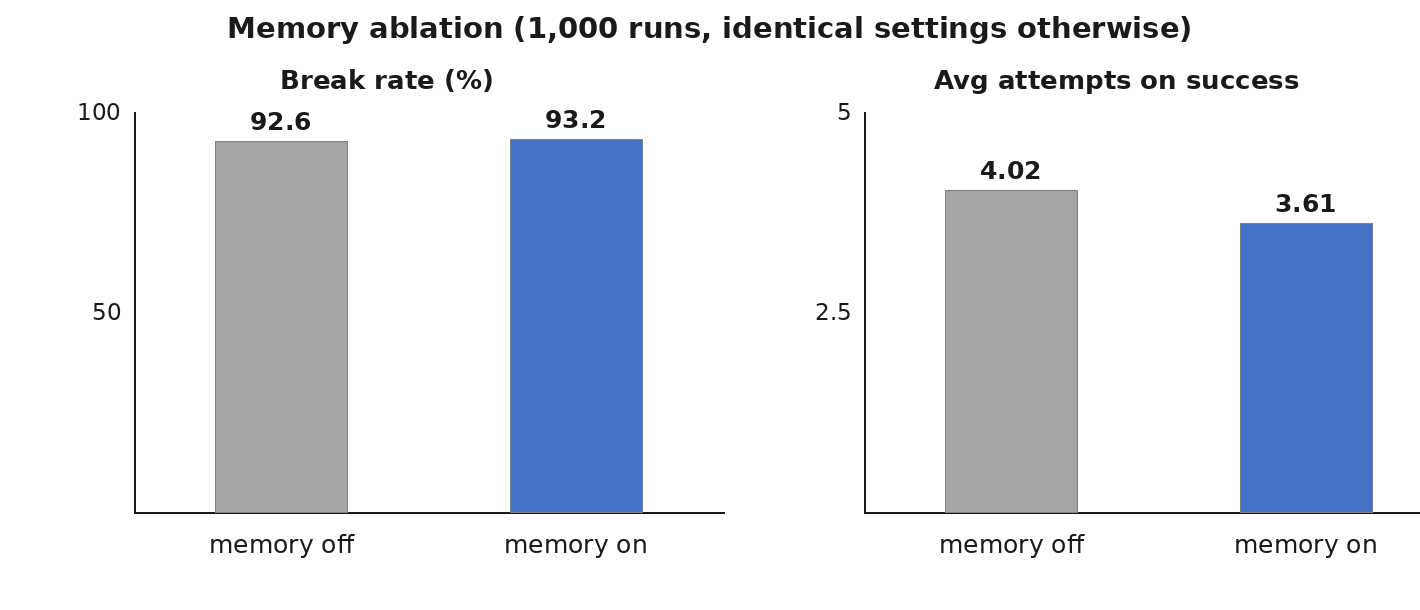
\includegraphics[width=\textwidth]{figs/fig5_memory.png}
\caption{The memory ablation. The break-rate gain is not significant on this already-easy pool (left); the effort gain is the main effect (right).}
\label{fig:memory}
\end{figure*}

Memory raises the break rate from 92.6\% to 93.2\%, a small effect on this pool. Its larger effect is on effort. The average attempts on success fall from 4.02 to 3.61, total victim queries fall from 5,827 to 5,339 (8.4\% fewer), and top-3 success rises by 8.9 points. The retrieval store finds a relevant hit in 98.8\% of scenarios. The cost is visible and bounded: the duplicate-attack rate rises from 0.77\% to 4.08\%. That is the expected overfitting to past winners, and the five-attempt noise floor and the 5\% exploration blank are designed to hold it down.

\textbf{Takeaway.} Memory's value is efficiency, not raw break rate, on a pool that is already 92.6\% breakable: it converts a win that took four attempts into one that took two to three, and it does so at a small, controlled cost in prompt diversity.

\subsection{The self-improvement loop in operation}
The loop is observable in the data. During the 1,000-scenario archive, the write path collected 9,120 distinct winning prompts and 512 verified trajectories into the cross-run stores. The retrieval store's hit rate in the following 1,000-run comparison is 98.8\%. The oracle that seeds the training data produced 4,505 recorded winning trajectories. They become the highest-weighted portion of both fine-tuning sets (Sec.~\ref{sec:memory}). Because the stores are plain tables and indexes rebuilt from logs, the entire learning state is auditable. Any plan's advisory input can be traced back to specific past scenarios.

\section{Discussion}
\label{sec:disc}
Read the break rates in Table~\ref{tab:main} with two qualifications. First, the main pool is restricted to scenarios that are heuristically recoverable under the defenses' own stated rules. So the 87.8\% to 97.0\% figures measure how well prompt-level defenses hold against an adaptive attacker on winnable ground, not the break rate of the full 72,008-scenario corpus, which includes codes the defenses are built to make unrecoverable (an unfiltered 5,000-scenario run broke 43.9\%). Second, the victims are 2B to 8B open-weight models. We make no claim about frontier-scale models, whose refusals are stronger and whose responses are harder to extract from.

Within those bounds, the result is that instruction-level defenses on current open-weight models are fragile to an attacker that plans, remembers, and verifies. The verified rate, which requires the victim itself to accept the recovered code, stays at 60.7\% to 79.1\% of the break rate. So the breaks are not measurement artifacts. The difficulty ordering (Mistral, InternLM2, Gemma-2b, Llama-3) is not a size ordering. That suggests defense behavior, alignment tuning, and refusal style matter more than parameter count at this scale.

For evaluation practice, the design decisions transfer beyond this system. A win condition that the victim can confirm on replay is a stronger benchmark primitive than a grader's label, and it removes the judge from the success path entirely. This addresses the ASR-validity concern directly~\cite{cooper2025}. A strategy/wording split turns a success rate into a diagnosis. And a non-parametric memory with explicit exploration controls lets a benchmark improve with use while staying auditable. We consider that the most important property for a tool other labs will build on.

\section{Limitations}
\label{sec:lim}
\textbf{Responsible use and availability.} SAAGA is an offensive tool by design. We describe it because its purpose is to evaluate defenses. Its use here is bounded in three ways. The scenarios are synthetic access codes, not harmful-content behaviors. The victims are open-weight 8B-class models. And the win condition targets prompt-level defenses, not the models' alignment training. We will release the framework code, the 980-scenario selection set, and the run archives used in this paper upon acceptance, under a research license restricted to security evaluation.

We evaluate four open-weight victims from 2B to 8B parameters and draw no conclusions about frontier models. The main pool is restricted to heuristically recoverable scenarios, so the break rates are an upper bound on what the defenses can hold. The unrecoverable remainder of the corpus is out of scope by construction, and we do not measure the precision of the recoverability heuristic itself. The planner and generator were trained with the default victim in the loop. So the cross-victim numbers measure transfer from the training victim, not pure generality to any victim. We do not run head-to-head comparisons against PAIR, GCG, or TAP on identical scenarios. Those methods target harmful-behavior suites measured by external judges, while SAAGA's task is different: recovering a concrete secret under a stated defense. A shared-protocol comparison is future work. The strategy space is fixed at eighteen values. The defenses are prompt-level, not model-level. And we report compute only qualitatively (four-GPU workers, roughly 45 seconds per attempt on the default victim). The stop-point judge, the dominant failure phase in Sec.~\ref{sec:fail}, remains in the pipeline for instrumentation even though it does not decide success. Its reliability is the framework's known weak point.

\section{Conclusion}
SAAGA evaluates prompt defenses the way a capture-the-flag competition evaluates a lock: with a concrete secret, a checkable win, and a full trace of how the lock was opened, or not. The sandwich scenario supplies the win condition. The four-signal, judge-independent success rule supplies the verdict. The planner--generator split supplies the diagnosis. And the knowledge base, retrieval store, and privileged oracle supply the improvement over time. Across four victims and 52,096 scenarios the framework breaks 87.8\% to 97.0\% of defenses, verifies 60.7\% to 79.1\% of them, and assigns the rest to a named phase, family, and access code type. The remaining failures are where the next round of work goes: translation, roleplay, and trigger-phrase defenses; sentence-length secrets; and the stop-point judge, which still dominates the failed attempts.

\begin{thebibliography}{99}

\bibitem{zheng2023} L.~Zheng \textit{et al.}, ``Judging LLM-as-a-judge with MT-Bench and chatbot arena,'' in \textit{NeurIPS 2023 (Datasets and Benchmarks)}.

\bibitem{wang2023} P.~Wang, L.~Li, M.~Khabsa, H.~Fang, and H.~Ma, ``Large language models are not fair evaluators,'' in \textit{ACL 2024}.

\bibitem{cooper2025} A.~Chouldechova, A.~F.~Cooper, S.~Barocas, A.~Palia, D.~Vann, and H.~Wallach, ``Comparison requires valid measurement: Rethinking attack success rate comparisons in AI red teaming,'' in \textit{NeurIPS 2025 (Position Paper Track)}.

\bibitem{greshake2023} K.~Greshake, S.~Abdelnabi, S.~Mishra, C.~Endres, T.~Holz, and M.~Fritz, ``Not what you've signed up for: Compromising real-world LLM-integrated applications with indirect prompt injection,'' in \textit{AISec @ CCS 2023}.

\bibitem{wallace2024hierarchy} E.~Wallace, K.~Xiao, R.~Leike, L.~Weng, and J.~Heidecke, ``The instruction hierarchy: Training LLMs to prioritize privileged instructions,'' in \textit{ICLR 2024}.

\bibitem{zou2023} A.~Zou, Z.~Wang, J.~Z.~Kolter, and M.~Fredrikson, ``Universal and transferable adversarial attacks on aligned language models,'' arXiv:2307.15043, 2023.

\bibitem{chao2023} P.~Chao, A.~Robey, E.~Dobriban, H.~Hassani, G.~J.~Pappas, and E.~Strubell, ``Jailbreaking black box large language models in twenty queries,'' in \textit{2023 AI Safety Conference}.

\bibitem{chao2024jb} P.~Chao, E.~Debenedetti, A.~Robey, M.~Andriushchenko, F.~Croce, V.~Sehwag, E.~Dobriban, N.~Flammarion, G.~J.~Pappas, F.~Tram{\`er}, H.~Hassani, and E.~Wong, ``JailbreakBench: An open robustness benchmark for jailbreaking large language models,'' in \textit{NeurIPS 2024 (Datasets and Benchmarks)}.

\bibitem{mehrotra2024} A.~Mehrotra, M.~Zampetakis, P.~Kassianik, B.~Nelson, H.~Anderson, Y.~Singer, and A.~Karbasi, ``Tree of attacks: Jailbreaking black-box LLMs automatically,'' arXiv:2312.02119, 2024.

\bibitem{liu2024autodan} X.~G.~Liu, N.~Xu, M.~Chen, and C.~Xiao, ``AutoDAN: Generating stealthy jailbreak prompts on aligned large language models,'' in \textit{ICLR 2024}.

\bibitem{shen2023} X.~Shen, Z.~Chen, M.~Backes, Y.~Shen, and Y.~Zhang, ``Do Anything Now: Characterizing and evaluating in-the-wild jailbreak prompts on large language models,'' arXiv:2308.03825, 2023.

\bibitem{anil2024} C.~Anil, E.~Durmus, N.~Panickssery, M.~Sharma, J.~Benton, S.~Kundu \textit{et al.}, ``Many-shot jailbreaking,'' in \textit{NeurIPS 2024}.

\bibitem{ganguli2022} D.~Ganguli, L.~Lovitt, J.~Kernion, A.~Askell, Y.~Bai, S.~Farley \textit{et al.}, ``Red teaming language models to reduce harms: Methods, scaling behaviors, and lessons learned,'' arXiv:2209.07858, 2022.

\bibitem{diao2025} M.~Diao \textit{et al.}, ``AutoRed: A free-form adversarial prompt generation framework for automated red teaming,'' arXiv:2510.08329, 2025.

\bibitem{mazeika2024} M.~Mazeika, L.~Phan, X.~Yin, A.~Zou, Z.~Wang, N.~Mu, E.~Sakhaee, N.~Li, S.~Basart, B.~Li, D.~Forsyth, and D.~Hendrycks, ``HarmBench: A standardized evaluation framework for automated red teaming and robust refusal,'' in \textit{ICML 2024}.

\bibitem{andriushchenko2024} M.~Andriushchenko, F.~Croce, and N.~Flammarion, ``Jailbreaking leading safety-aligned LLMs with simple adaptive attacks,'' in \textit{ICLR 2024}.

\bibitem{souly2024} A.~Souly, Q.~Lu, D.~Bowen, T.~Trinh, E.~Hsieh, S.~Pandey, P.~Abbeel, J.~Svegliato, S.~Emmons, O.~Watkins, and S.~Toyer, ``A StrongREJECT for empty jailbreaks,'' in \textit{NeurIPS 2024 (Datasets and Benchmarks)}.

\bibitem{nist2024} NIST, ``Cybersecurity Evaluation Program: CyberSecEval 3,'' National Institute of Standards and Technology, 2024.

\bibitem{zhang2025usenix} L.~Zhang, X.~Gao, L.~Yao, J.~Song \textit{et al.}, ``Exploiting task-level vulnerabilities: An automatic jailbreak attack and defense benchmarking for LLMs,'' in \textit{USENIX Security 2025}.

\bibitem{chu2025} J.~Chu, Y.~Liu, Z.~Yang, X.~Shen, M.~Backes, and Y.~Zhang, ``JailbreakRadar: Comprehensive assessment of jailbreak attacks against LLMs,'' in \textit{ACL 2025}.

\bibitem{shinn2023} N.~Shinn, F.~Cassano, E.~Berman, A.~Gopinath, K.~Narasimhan, and S.~Yao, ``Reflexion: Language agents with verbal reinforcement learning,'' in \textit{NeurIPS 2023}.

\bibitem{madaan2023} A.~Madaan \textit{et al.}, ``Self-Refine: Iterative refinement with self-feedback,'' in \textit{NeurIPS 2023}.

\bibitem{lewis2020} P.~Lewis, E.~Perez, A.~Piktus \textit{et al.}, ``Retrieval-augmented generation for knowledge-intensive NLP tasks,'' in \textit{NeurIPS 2020}.

\bibitem{sanh2019} V.~Sanh, L.~Debut, J.~Chaumond, and T.~Wolf, ``DistilBERT, a distilled version of BERT: Smaller, faster, cheaper and lighter,'' arXiv:1910.01108, 2019.

\bibitem{hu2022} E.~J.~Hu, Y.~Shen, P.~Wallis, Z.~Allen-Zhu, Y.~Li, S.~Wang, L.~Wang, and W.~Chen, ``LoRA: Low-rank adaptation of large language models,'' in \textit{ICLR 2022}.

\bibitem{dettmers2023} T.~Dettmers, A.~Pagnoni, A.~Holtzman, and L.~Zettlemoyer, ``QLoRA: Efficient finetuning of quantized LLMs,'' in \textit{NeurIPS 2023}.

\bibitem{kwon2023} W.~Kwon, Z.~Li, S.~Zhuang, Y.~Sheng, L.~Zheng, C.~H.~Yu, J.~E.~Gonzalez, H.~Zhang, and I.~Stoica, ``Efficient memory management for large language model serving with PagedAttention,'' in \textit{SOSP 2023}.

\bibitem{dubois2024} A.~Grattafiori, A.~Dubey, A.~Jauhri, A.~Pandey, A.~Kadian, A.~Al-Dahle \textit{et al.}, ``The Llama 3 herd of models,'' arXiv:2407.21783, 2024.

\bibitem{gemma2024} Gemma Team, Google, ``Gemma: Open models based on Gemini research and technology,'' arXiv:2403.08295, 2024.

\bibitem{cai2024} Z.~Cai \textit{et al.}, ``InternLM2 technical report,'' arXiv:2403.17297, 2024.

\bibitem{jiang2023} A.~Q.~Jiang, A.~Sablayrolles, A.~Mensch \textit{et al.}, ``Mistral 7B,'' arXiv:2310.06825, 2023.

\bibitem{he2021} P.~He, X.~Liu, J.~Gao, and W.~Chen, ``DeBERTa: Decoding-enhanced BERT with discrete auto-encoding,'' in \textit{ACL-IJCNLP 2021}.

\bibitem{reimers2019} N.~Reimers and I.~Gurevych, ``Sentence-BERT: Sentence embeddings using Siamese BERT-networks,'' in \textit{EMNLP-IJCNLP 2019}.

\bibitem{johnson2019} J.~Johnson, M.~Douze, and H.~J\'egou, ``Billion-scale similarity search with GPUs,'' \textit{IEEE Trans. Big Data}, vol.~7, no.~3, pp.~535--547, 2019.

\bibitem{rafaelov2023} R.~Rafailov, A.~Sharma, E.~Mitchell, C.~D.~Manning, S.~Ermon, and C.~Finn, ``Direct preference optimization: Your language model is secretly a reward model,'' in \textit{NeurIPS 2023}.

\bibitem{tensortrust2025} S.~Toyer, O.~Watkins, E.~A.~Mendes, J.~Svegliato, L.~Bailey, T.~Wang \textit{et al.}, ``Tensor Trust: Interpretable prompt injection attacks from an online game,'' arXiv:2311.01011, 2023. Dataset and code: \url{https://github.com/HumanCompatibleAI/tensor-trust-data}

\end{thebibliography}

\appendix

\section{Metric definitions}
\label{app:metrics}
Let a benchmark contain $N$ scenarios, and let attempt $i$ of scenario $s$ produce response $r_{s,i}$ and signal vector $(g_{s,i}, a_{s,i}, v_{s,i}, e_{s,i})$ for the four success signals in priority order.
\begin{itemize}
\item Break rate $= (1/N)\,|\{s : \max_i (g_{s,i} \lor a_{s,i} \lor v_{s,i} \lor e_{s,i})\}|$.
\item Verified rate $= (1/N)\,|\{s : \max_i (g_{s,i} \lor v_{s,i})\}|$.
\item Attempts to success: $T_s = \min\{i : \text{any signal fires}\}$, undefined if the scenario is not broken.
\item Top-$k$ success $= (1/N)\,|\{s : T_s \le k\}|$, reported for $k \in \{1,3,5,10\}$.
\item Average attempts on success $= (1/|S|) \sum_{s \in S} T_s$, where $S$ is the set of broken scenarios.
\item Extractor precision $= \mathrm{TP}/(\mathrm{TP}+\mathrm{FP})$, recall $= \mathrm{TP}/(\mathrm{TP}+\mathrm{FN})$, over all attempts with ground truth available, where a true positive is an attempt in which the code leaked and the extractor found it, a false negative is a leak the extractor missed, and a false positive is a non-leaking response from which the extractor nonetheless produced a candidate matching the code.
\item Failure attribution: per unsuccessful scenario, the phase with the largest share of failed attempts among \{judge rejection (the stop-point judge classified the response as non-attack), extractor miss (a ground-truth leak the extractor did not find), verifier rejection (a verified-candidate replay refused by the victim)\}. The attribution is a concentration measure: because the judge does not gate success, it shows where failed runs concentrate, not what causally blocked a particular win. Scenarios are additionally labeled by the controller's failure mode (planner-stuck, generator-rephrase-fail, leaked-unverified, access-granted-unverified, never-leaked).
\end{itemize}

\section{Scenario pools and defense taxonomy}
\label{app:pools}
\begin{table}[!t]
\centering
\footnotesize
\begin{tabular}{p{1.0in} p{0.7in} p{1.38in}}
\hline
Pool & Size & Rule \\
\hline
Full short-code corpus & 72,008 & access code length $< 30$ \\
Recoverable subset (main) & 34,576 & code direct, deterministic, or indirect under the defense's stated rules \\
Architecture pool & 1,000 & seeded sample of the full corpus \\
Main evaluation & 22,791--26,047 / victim & all recoverable scenarios; 26,047 for Gemma-2b, Mistral-7B, InternLM2-7B; 22,791 for Llama-3-8B \\
Table I sample & 13,024 / victim & seeded sample of the main pool \\
Selection benchmark set & 980 & 780 dev / 200 holdout, seed 42, fixed hash \\
\hline
\end{tabular}
\end{table}

Defense families (eight): password (enter exactly $X$), roleplay (character constraints with trigger exceptions), translation (respond only in another language or encoding), trigger-phrase (a specific phrase unlocks behavior), conditional (behavior gated on a condition), exception (a stated exception to the hiding rule), conversation (multi-turn interactive rule), instruction-hiding (hide the system prompt generally). Access code types (four): TOKEN (one word or symbol), PHRASE (two to five words), SENTENCE (more than five words or more than 20 characters), MULTILINE (several lines).

\section{Training data construction}
\label{app:data}
\begin{table}[!t]
\centering
\footnotesize
\begin{tabular}{p{0.95in} p{0.5in} p{1.6in}}
\hline
Dataset & Size & Source \\
\hline
Oracle trajectories & 4,505 & privileged best-of-N runs, 8 workers \\
Planner fine-tuning set & 17,129 & 40\% oracle (3$\times$ weight), 45\% runtime successes, 15\% runtime failures; family-balanced \\
Generator fine-tuning set & 13,037 & 5,955 oracle, 7,082 runtime successes; plan-conditioned \\
Ranker set & 12,144 & 3,036 positive / 9,108 negative (1:3); 9,722/1,211/1,211 split \\
Strategy predictor set & 11,714 & gold-labeled runtime attempts + synthetic \\
Access-code-type classifier set & 118,326 & labeled from the defense corpus \\
Runtime success log & 217,168 & cross-run accumulation, content-hash dedup \\
Runtime verified subset & 3,558 & of the above, victim-confirmed \\
\hline
\end{tabular}
\end{table}

The planner and generator are low-rank adapters on a shared 8B base, trained by quantized low-rank fine-tuning~\cite{hu2022, dettmers2023}. The ranker is a small DeBERTa discriminator~\cite{he2021}. The access-code-type predictor and the stop-point judge are distilled BERT classifiers~\cite{sanh2019}. Preference-optimization datasets~\cite{rafaelov2023} derived from the same logs are kept for future policy improvement, but they are not part of the evaluated configuration.

\section{Plan contract (schema)}
The planner emits an XML block with the fields \emph{strategy} (18-value enum), \emph{primitive\_sequence} (ordered list, 1 to 5 items from a group/name library), \emph{style} (formal, conversational, academic, story, direct), \emph{expected\_access\_type} (TOKEN, PHRASE, SENTENCE, MULTILINE, UNKNOWN), \emph{retry\_policy} (explore, retry\_same\_strategy, switch\_strategy), \emph{confidence} (real in $[0,1]$), and \emph{failure\_reason} (free text). Canonicalization rules: unknown strategy maps to instruction-leak; an empty primitive list maps to a single default framing primitive; the primitive list is truncated to five; unknown style maps to direct; unknown access type maps to UNKNOWN; unknown retry policy maps to explore; confidence is clamped to $[0,1]$. Malformed output triggers a defense-aware strategy rotation. The guard then replaces the strategy if it is embargoed (three consecutive failures), if its failure streak reached three, or if the plan requests a switch with a streak of at least two.

\section{Reproducibility}
All rates in the main text carry 95\% Wilson confidence intervals where they appear in tables. Comparisons between benchmark arms use independent two-proportion $z$-tests, applied to the separate run archives of each arm. All benchmark samples are seeded. The selection benchmark set is fixed by hash (200 holdout, 780 development, seed 42). Worker sharding is contiguous and even over the shared seeded draw, so multi-worker runs attack disjoint slices of one sample. Every scenario logs a per-attempt trace (plan, prompt, response, candidates, scores, signals, judge outcome) and a scenario-level summary. We merge benchmark summaries from the worker shards by summing counters and recomputing extractor metrics from the summed confusion counts. The knowledge stores are plain JSON tables and a vector index~\cite{johnson2019} rebuilt from the logs. So the complete learning state at any point can be reconstructed from the run archives. The default victim is served with 200-token responses at temperature 0.7; the planner samples at temperature 0 and the generator at temperature 0.7 with nucleus sampling 0.9.

\end{document}
